\chapterimage{golden_gate.jpg}

\chapter{Layer 3: Internet(work) communication}\label{sec:layer3}

\begin{minipage}{0.4\linewidth}
\begin{center}
\begin{bytefield}{16}
\bitbox{16}{Layer 7: Application} \\
\bitbox{16}{Layer 4: Transport} \\
\bitbox{16}{\color{color1} Layer 3: Internet} \\
\bitbox{16}{Layer 2: Network (LAN)} \\
\bitbox{16}{Layer 1: Physical} \\
\end{bytefield}
\end{center}
\end{minipage}
\begin{minipage}{0.6\linewidth}
\begin{center}
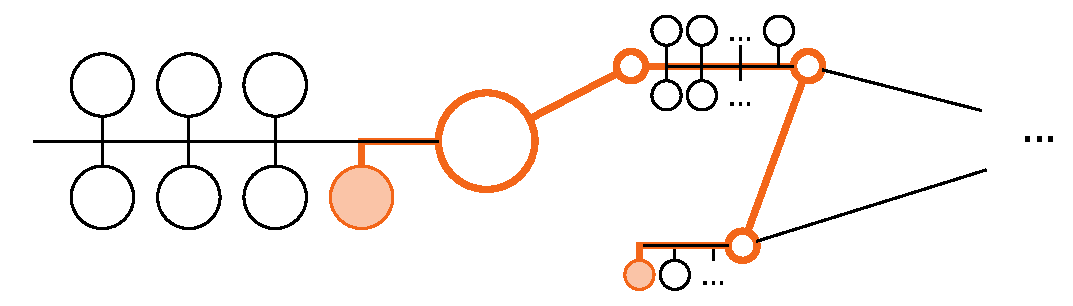
\includegraphics[width=\linewidth]{network_layer3.pdf}
\end{center}
\end{minipage}

\vspace{-0.75cm}


% \section{Layer~3 overview}
\subsection*{Capabilities}

The \conceptRef{IP}{Internet Protocol (IP)} allows exchanging \concept{datagrams} 
(Layer~3 \conceptRef{PDU}{PDUs}) between devices from different \conceptRef{LAN}{LANs}.
% 
Its addressing system identifies devices globally and makes it possible to 
\conceptRef{routing}{route} datagrams anywhere we need. 

Devices communicating via IP may belong to LANs
based on different technologies and with different types of \concept{MAC} address.
This has two implications:
\begin{itemize}
  \item A datagram that ``fits'' in the \concept{MTU} of the source LAN
    may be too large for the destination's (or any intermediate's) LAN MTU. 
    IP defines a \concept{fragmentation} system to split datagrams,
    which are reconstructed only at the final destination.\\[-0.25cm]
    
  \item When we send a datagram, we know the target device's \conceptRef{IP}{IP address},
  but not necessarily its \concept{MAC} address. Only if we are part of the destination
  LAN we will need that MAC. IP uses \concept{ARP} to translate known IP addresses
  to MAC addresses of the destination LAN's type.
\end{itemize}


\conceptRef{datagram}{Datagrams} may travel through networks not controlled 
by neither the source nor the destination, so datagrams may be lost, reordered and duplicated.
% 
Layer~3 does not provide mechanisms to deal with this; upper layers must implement
protection mechanisms when required 
(\eg, to implement \concept{TCP}'s \conceptRef{stream}{data streams}).

\begin{center}
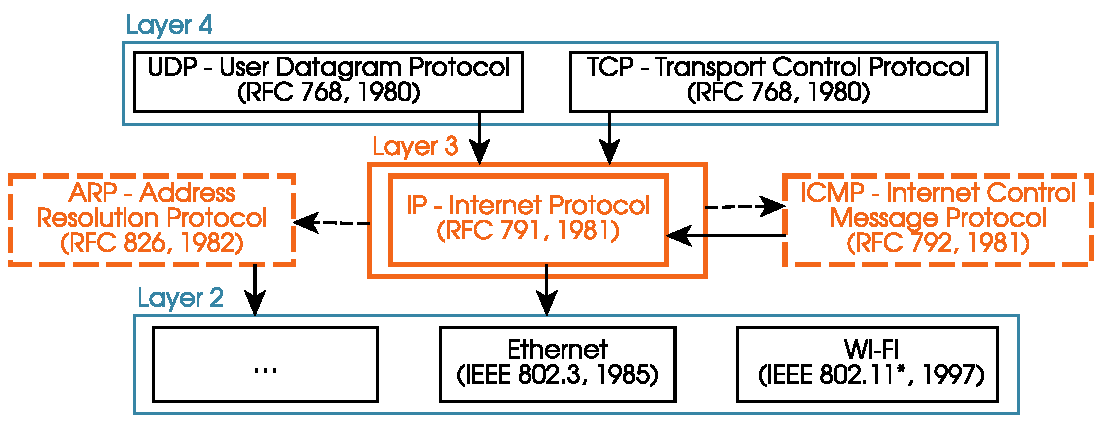
\includegraphics[width=0.9\linewidth]{protocols_layer3.pdf}
\end{center}


\vspace{-0.25cm}
\subsection*{Protocols}

Version~4 of \concept{IP} is \textit{the} protocol used in Layer~3, \ie,
it is common to virtually all communications in the Internet as we know it today.
% 
For many years, the Internet has been struggling to transition towards \concept{IPv6}, 
but the process is not complete and only \concept{IPv4} provides global coverage.

\concept{IPv4} delegates in the \concept{ARP} protocol the translation of known IP addresses 
into MAC addresses within each LAN. ARP does \textit{not} use IP datagrams.

The following protocols encapsulate their \conceptRef{PDU}{PDUs} in the payload of IP 
\conceptRef{datagram}{datagrams}:\\[-0.6cm]
\begin{itemize}
\item Transport Control Protocol (\concept{TCP}) 
\item User Datagram Protocol (\concept{UDP})
\item Internet Control Message Protocol (\concept{ICMP})
\end{itemize}

\begin{remark}
The \inlineCode{ip address}, \inlineCode{ip route} and \inlineCode{ip neighbor} commands 
(among others) let you query several aspects of your IP configuration.
\end{remark}



\section{Layer~3 addressing}

\concept{IPv4} addresses are $32$~bits long. They are most often presented to humans in
the \concept{quad decimal} format, \eg,
\begin{center}
\otherBase{142.250.201.67}
\end{center}

\concept{IPv6} addresses are $128$~bits ($12$~bytes) long, \ie, 
they are $4$~times larger than an IPv4 address.
They are expressed in hexadecimal format, \eg, as follows. Note how 
two colon signs ``\otherBase{::}'' indicate ``fill with zeros'',
and ``\otherBase{::}'' may only appear once per IPv6 address.
\begin{center}
\otherBase{fe80::f524:a73a:e946:7c02}
\end{center}

\begin{remark}
When an \concept{IPv6} address is used as part of an URL, it is surrounded with brackets,
\eg, \otherBase{https://[fe80::f524:a73a:e946:7c02]/}.
\end{remark}


\subsection{Public and reserved addresses}

Most IP addresses are \conceptRef{public IP}{public} and unique across the Internet, 
\ie, the previous IP has the same meaning worldwide: it identifies a single connected device.
% 
Many addresses are \conceptRef{reserved IP address}{reserved/private} and can only be 
used within a particular scope (\eg, a LAN) or situation.
Some of the most common are the following (there are 
\href{https://en.wikipedia.org/wiki/Reserved_IP_addresses#IPv4}{\underline{some more}}, 
also for IPv6):

\begin{center}
\begin{tabular}{ll}
\toprule
\textbf{IP address block} & \textbf{Address scope} \\
\toprule
\otherBase{127.*.*.*} & This computer (localhost) \\[0.1cm]
\otherBase{10.*.*.*} & This LAN \\
\otherBase{172.16.*.*} & This LAN \\
\otherBase{192.168.*.*} & This LAN \\[0.1cm]
\otherBase{0.*.*.*} & Special usages \\
\otherBase{169.254.*.*}& Special usages \\
\otherBase{255.255.255.255} & Special usages\\
\bottomrule
\end{tabular}
\end{center}

\begin{exercise}\ \\[-0.5cm]
\begin{itemize}
\item How many different \concept{IPv4} addresses are there (including reserved and private)? 
\item Are they sufficient now and in the future?
\item Is it problematic that an address like \otherBase{192.168.0.1} 
  is simultaneously used by thousands (likely millions) of computers in the Internet right now?
\end{itemize}
\end{exercise}

\subsection{Netmasks}\label{sec:layer3:netmasks}

The $32$~bits of an IP address can be divided in two parts using a \concept{netmask}:\\[-0.25cm]
% 
\begin{center}
\begin{bytefield}{32}
\bitheader{0-31}\\
\bitbox{10}{Network ID} & \bitbox{22}{Device ID} \\
\end{bytefield}
\end{center}
% 
The first part identifies the LAN or group of LANs to which a device belongs. 
The second part identifies a single device in the LAN. 
The netmask determines how many bits are assigned to each part. 

In the previous figure, the netmask assigns 10 bits to the network ID and 22 to the device ID.
This mask can be anywhere from $0$ (all bits are device ID) to $32$ (all bits are network ID).


Netmasks are presented to humans in two main ways:\\[-0.5cm]
\begin{itemize}
  \item \otherBase{/N}, where $N$ is the number of bits assigned to the Network ID. 
    This is used in the \concept{CIDR} format.
  
  \item The \concept{quad decimal} (\otherBase{A.B.C.D}) format of 
    $N$ bits set to \otherBase{1}, followed by $(32-N)$ bits set to \otherBase{0}.
\end{itemize}

\begin{exercise}
The netmask of the previous example can be expressed in binary 
(although it is not very convenient):
\begin{center}
\begin{bytefield}[bitwidth=1em]{32}
\bitheader{0-31} \\
\bitboxes{1}{1111111111} &
\bitboxes{1}{0000000000 0000000000 00} \\
\bitbox{10}{$10$~bits} & \bitbox{22}{$32-N = 22$~bits}
\end{bytefield}
\end{center}

\begin{itemize}
\item Express the netmask of the previous example in the CIDR and quad decimal formats.
\item What is your IP and netmask? Express it in the same two main ways.
\end{itemize}
\end{exercise}

\begin{remark}
Netmasks are used in IPv6 as well, but with a maximum value of $N$ of $128$ instead of $32$.
\end{remark}

\subsection{Blocks of IP addresses}

Netmasks are used in combination with IP addresses to define 
\conceptRef{IP address block}{blocks of IP addresses} 
that begin with the same $N$ bits (where $N$ is the netmask).
% 
For instance, \otherBase{192.168.3.0/24} (in \concept{CIDR} format) 
and \otherBase{192.168.3.0/255.255.255.0} refer to the block 
of addresses between \otherBase{192.168.3.0} and \otherBase{192.168.3.255},
both included
(\otherBase{192.168.3.*} in the informal notation of the previous table).

\begin{exercise} 
IP blocks can be smaller than, equal to or larger than an IP network.
Provide examples where an IP block refers to:
\begin{itemize}
\item A single IP.
\item Half the IP addresses in the \otherBase{192.168.3.0/24} network.
\item All addresses of the \otherBase{192.168.3.0/24} network, plus 
      $256$ more addresses.
\item All possible IPs.
\end{itemize}
\end{exercise}


\begin{exercise}\ \\[-0.65cm]
\begin{itemize}
\item Can every \concept{netmask} be expressed as an \concept{IP address}?
\item List all possible netmasks.\\[-0.5cm]
\end{itemize}
\end{exercise}

When referring to a block of addresses (like a LAN), 
the IP address in this IP + netmask combination
must have all device ID bits set to \otherBase{0}. 
This way, \otherBase{192.168.3.0/24} correctly refers to a network, but
\otherBase{192.168.3.1/24} refers instead to a device 
(the one with IP \otherBase{192.168.3.1}) in that network (\otherBase{192.168.3.0/24}).

\subsection{LANs and netmasks}\label{sec:layer3:lans_and_netmasks}

Netmasks need \textit{not} be multiples of $8$. Consider the following example in which \\
\otherBase{192.168.76.1/19} (a device's IP + netmask) is used to obtain its network address\\
(\otherBase{192.168.64.0/19}):\\

\begin{center}
\begin{bytefield}[bitwidth=1.1em]{32}
\bitheader{0-31}\\
\begin{rightwordgroup}{Device's IP}
\bitbox{8}{192} & \bitbox{8}{168} & \bitbox{8}{76} &\bitbox{8}{1} \\
\bitboxes{1}{11000000} & \bitboxes{1}{10101000} & \bitboxes{1}{0100{\bf1}{\bf1}00} & \bitboxes{1}{0000000{\bf1}}
\end{rightwordgroup} \\

\bitboxes[]{1}{\&\&\&\& \&\&\&\& \&\&\&\& \&\&\&\& \&\&\&
               {\color{color1}\&} 
               {\color{color1}\&}{\color{color1}\&}{\color{color1}\&}{\color{color1}\&}
               {\color{color1}\&}{\color{color1}\&}{\color{color1}\&}{\color{color1}\&}
               {\color{color1}\&}{\color{color1}\&}{\color{color1}\&}{\color{color1}\&}} \\

\begin{rightwordgroup}{Netmask}
\bitboxes{1}{1111111111111111111
   {\color{color1}0}{\color{color1}0}{\color{color1}0}{\color{color1}0}
   {\color{color1}0}{\color{color1}0}{\color{color1}0}{\color{color1}0}
   {\color{color1}0}{\color{color1}0}{\color{color1}0}{\color{color1}0}
   {\color{color1}0}}
\end{rightwordgroup} \\

\bitboxes[]{1}{==== ==== ==== ==== ===
               {\color{color1}=} 
               {\color{color1}=}{\color{color1}=}{\color{color1}=}{\color{color1}=}
               {\color{color1}=}{\color{color1}=}{\color{color1}=}{\color{color1}=}
               {\color{color1}=}{\color{color1}=}{\color{color1}=}{\color{color1}=}} \\

\begin{rightwordgroup}{Network IP}
\bitboxes{1}{11000000} & \bitboxes{1}{10101000} & \bitboxes{1}{0100{\bf0}{\bf0}00} & \bitboxes{1}{0000000{\bf0}} \\
\bitbox{8}{192} & \bitbox{8}{168} & \bitbox{8}{64} &\bitbox{8}{0} 
\end{rightwordgroup}\\
\end{bytefield}
\end{center}

\begin{exercise}\ \\[-0.5cm]
\begin{itemize}
\item In the previous example, we only really needed to transform one decimal value to binary,
and one decimal value to binary. Which one?
\item Is this always true when converting IP+netmask combinations to network addresses?
\item Express the netmask in \concept{quad decimal} format.
\end{itemize}
\end{exercise}



Given a IP + netmask address block and a device's IP address, it is direct to determine 
whether that device's IP belongs to the block (if and only if the first $N$ bits match,
where \otherBase{/N} is the CIDR netmask).

\begin{exercise}
Determine whether each of the following addresses belong to the same network as
the following device \otherBase{123.45.67.89/14}:
\begin{itemize}
\item \otherBase{23.45.67.89}
\item \otherBase{123.45.203.25}
\item \otherBase{123.43.255.255}
\item \otherBase{0.45.67.1}
\end{itemize}
\end{exercise}

An \conceptRef{network}{IP network} (a LAN) is a block of addresses, but not all those addresses 
can be assigned to devices. Two addresses are always reserved:
\begin{itemize}
\item The address with all node bits set to \otherBase{0}: it identifies the LAN itself.
\item The address with all node bits set to \otherBase{1}: it identifies \concept{broadcast} within the LAN.
\end{itemize}

\begin{exercise}\ \\[-0.5cm]
\begin{itemize}
\item List all addresses that can be assigned to devices in \otherBase{192.168.54.0/29}.
\item List the broadcast address of that network.
\end{itemize}
\end{exercise}

The netmask \otherBase{/N} determines the number of devices that can be connected at the same time
to a network: $2^{32-N} - 2$. When LANs are called ``small'' or ``larger'', the size refers to that 
number of available device addresses. 

Conversely, the number $M$ of devices that we need to connect to the same LAN determines the 
smallest LAN size (largest netmask \otherBase{/N}) that fits all those devices at the same time:

\begin{center}
\begin{tabular}{ccc}
\toprule
\textbf{Netmask} & \textbf{Total addresses} & \textbf{Max devices} \\
\otherBase{/N} & $2^{32-N}$ & $2^{32-N} - 2$ \\
\toprule
\otherBase{/30} & 4 & 2 \\
\otherBase{/29} & 8 & 6 \\
\otherBase{/28} & 16 & 14 \\
\otherBase{/27} & 32 & 30 \\
\otherBase{/26} & 64 & 62 \\
\otherBase{/25} & 128 & 126 \\
$\vdots$ & $\vdots$ & $\vdots$ \\
\bottomrule
\end{tabular}
\end{center}

\begin{remark}
All \conceptRef{router}{routers} need a valid IP address per LAN to which they are connected.
Therefore, routers \textit{do} count towards the maximum number of devices connected in a LAN.
\end{remark}

\begin{exercise} \ \\[-0.5cm]
\begin{itemize}
\item What's the minimum network size that fits $256$ connected devices?
\item What's the longest netmask \otherBase{/N} that would let everyone in your city connect?
\item How many addresses are contained in a \otherBase{/0} network? 
\item How many \otherBase{/0} networks may exist? Are they given names?
\end{itemize}
\end{exercise}


\begin{exercise}
The following code snippet takes an IP address and shows its $4$~bytes expressed in 
quad decimal and in binary.
Extend (or replace) the code so that you can:
\begin{itemize}
\item Transform $32$ bits into a quad decimal string.
\item Display a netmask in IP address and CIDR formats.
\item Given a device's IP and netmask, determine whether other IP belongs to the same network.
\end{itemize}
\begin{center}
\showCode{snippets/ipcalculator.py}
\end{center}
\end{exercise}




% \todo{exercise netmask calculator}
% 
% \todo{HERE HERE HERE: add and point to the subnetting area}







\section{IP -- Internet Protocol}

\subsection{Packet format}\label{sec:layer3:ip:format}

\concept{IP} defines a \concept{packet} format with a \concept{header} 
that is \textit{at least} $20$~bytes long. Optional parts may be included,
as long as the total header size is a multiple of $32$~bits ($4$~bytes).
The payload can be empty, so the minimum datagram size is $20$~bytes.\\

\begin{center}
\small
\begin{bytefield}[bitheight=3.4em,bitwidth=1.1em]{32}
\bitheader{0-31}\\
\begin{rightwordgroup}[curlyshrinkage=10pt]{Mandatory Header\\($20$~bytes)}
  \bitbox{4}{IP\\Version} 
  & \bitbox{4}{IHL\\{\scriptsize(HLen/$4$)}} 
  & \bitbox{8}{Type of Service}
  & \bitbox{16}{Datagram Length\\{\scriptsize(Head + Payload, bytes)}} \\
  % 
  \bitbox{16}{Fragment ID} & \bitbox{1}{\otherBase{0}}
  & \bitbox{1}{\rotatebox{90}{\scriptsize DF flag}}
  & \bitbox{1}{\rotatebox{90}{\scriptsize MF flag}}
  & \bitbox{13}{Fragment Offset} \\
  % 
  \bitbox{8}{Time to Live\\(TTL)}
  & \bitbox{8}{Payload protocol}
  & \bitbox{16}{IP Header Checksum}\\
  % 
  \bitbox{32}{Source IP Address} \\
  \bitbox{32}{Destination IP Address}
\end{rightwordgroup} \\
%   
\begin{rightwordgroup}[curlyshrinkage=10pt]{Optional Header\\{\scriptsize($4$ byte words)}}
\bitbox[tlr]{32}{Options\\{\scriptsize(variable length, optional)}} \\
\bitbox[lbr]{24}{} &
\bitbox{8}{Padding to\\$32$ bits}
\end{rightwordgroup} \\
% 
\begin{rightwordgroup}[curlyshrinkage=10pt]{Payload}
\bitbox[tlr]{32}[bitheight=3em]{Payload data\\{\scriptsize(variable length, byte aligned)}} \\
\bitbox[lbr]{24}{\hspace{3cm}\raisebox{0.25cm}{$\vdots$}} & \bitbox[lt]{8}{}
\end{rightwordgroup}
\end{bytefield}
\end{center}

\begin{exercise} \ \\[-0.5cm]
\begin{itemize}
\item How can the payload length be calculated from the header?
\item What is the maximum payload length?
\item What are the possible values of the flags in the IP header?
\item What's longer, an IP address or an Ethernet MAC address?
\item Is it possible to send exactly 17 bits of payload data in an IP datagram?
\item How can we know whether a datagram is encapsulating TCP or UDP data?
\item Why must the optional header part by a multiple of $32$~bits?
\end{itemize}
\end{exercise}

\subsection{Operation}

When a device A wants to send an IP datagram to a device B, the source and 
destination IPs in the header are fixed and don't change for this datagram.

If devices A and B belong to the same LAN, the datagram is sent directly
(\eg, encapsulated in an Ethernet frame). However, IP can go much farther.
Consider the following scenario, where A wants to communicate with E.

\begin{center}
 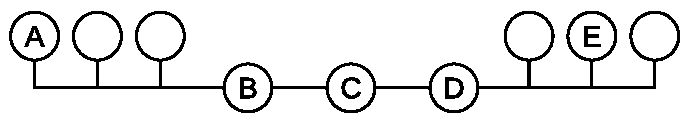
\includegraphics[width=0.5\linewidth]{ip_operation_example.pdf}
\end{center}


Here, the source and destination devices belong to different LANs.
The datagram is passed first to the source's \concept{router}.
Then, each intermediate router passes it to the next one until the datagram reaches 
the last router, which is connected to the destination LAN. Finally, that last router 
passes the datagram to the destination. 

\begin{center}
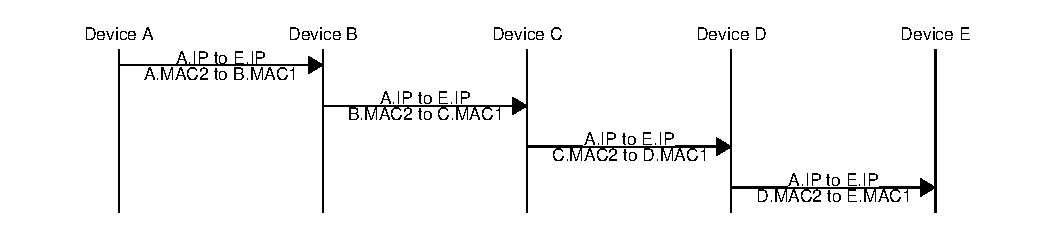
\includegraphics{ip_operation.eps}
\end{center}

The source and destination IP addresses don't change throughout the journey.
In contrast, MAC address change in each LAN \concept{hop}. 

\section{IP routing}\label{sec:layer3:routing}

\conceptRef{router}{Routers} are the devices in charge of forwarding IP \conceptRef{datagram}{datagrams}
by looking at the destination IP address of each one, present in the IP \concept{header}. Routers don't need 
to \concept{decapsulate} headers of layers 4 and above. Therefore, they network stacks need contain only up to Layer~3
(and so are sometimes referred to as Layer-3 devices).

\begin{center}
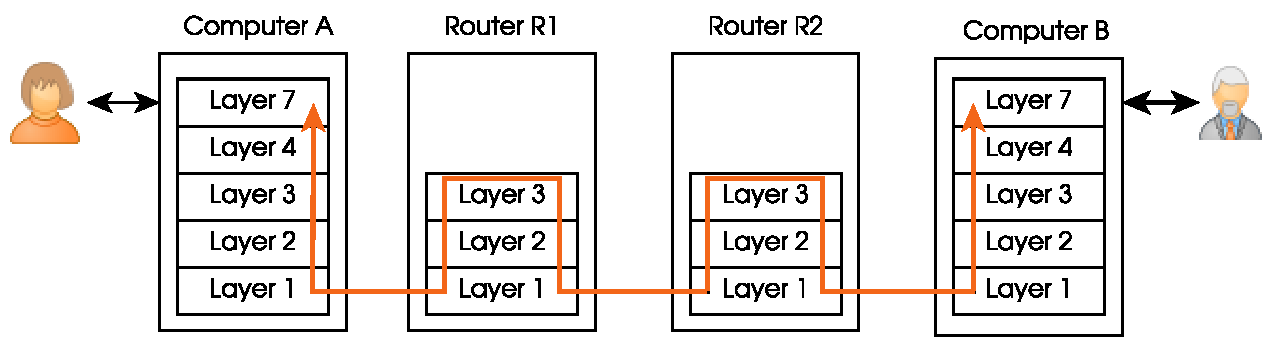
\includegraphics[width=0.9\linewidth]{forward_layers.pdf}
\end{center}


When a router detects a network frame $F$ in one of its \conceptRef{interface}{interfaces} (network cards),
it tries to recognize the following parts of a datagram.
\begin{center}
\begin{bytefield}{48}
\bitbox{12}{Layer~2 header} & \bitbox{12}{IP header} & \bitbox{24}{Datagram payload}
\end{bytefield}
\end{center}
If recognized, the router processes the datagram as follows:
\begin{enumerate}
\item The whole frame $F$ is discarded unless the destination MAC (in the Layer~2 header) 
  is that of the router's interface that detected the frame.\\[-0.25cm]
  
\item The router looks at the destination IP address (in the IP header of $F$) and at its \concept{routing table} 
  to decide the next \concept{hop} of the datagram, \ie, the device to which this router will pass 
  the datagram to, and what \concept{interface} to use (see Section~\ref{sec:layer3:routing} below).\\[-0.25cm]
  
\item The router creates and sends a frame $F'$ making the following two changes to $F$:\\[-0.25cm]
  \begin{enumerate}[label=\alph*)]
  \item The Layer~2 header in $F'$ changes entirely:
    \begin{itemize} 
    \item The destination \concept{MAC} is that of the next hop,
    and the source MAC is that of the router forwarding the datagram.
    The next hop's IP is given by the \concept{routing table} (see Section~\ref{sec:layer3:routing}), 
    and its MAC is obtained from that IP using \concept{ARP} (Section~\ref{sec:layer3:arp}).\\[-0.4cm]
    %     
    \item The source MAC of $F'$
    frame is different from the destination MAC of the received frame $F$ if the router 
    received $F$ in one interface (\eg \inlineCode{eth7}) and forwards it through another 
    (\eg,  \inlineCode{eth9}).
    \end{itemize}
    
    \begin{center}     
    \vspace{0.15cm}
    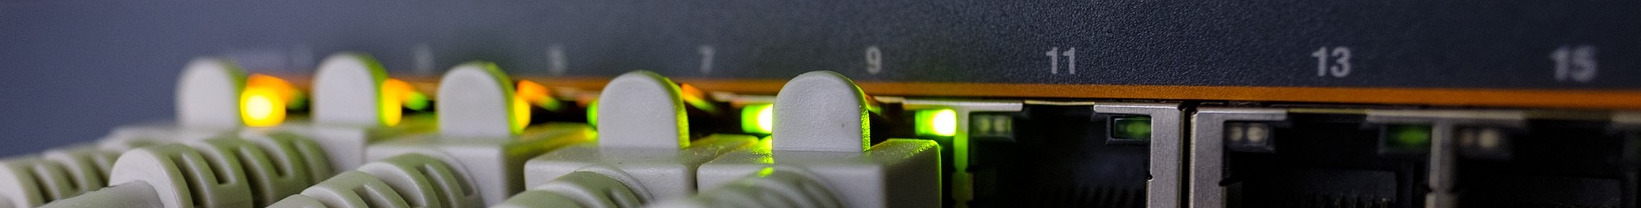
\includegraphics[width=0.8\linewidth]{router_ports.jpg}
    \vspace{0.15cm}
    \end{center}
    
  \item The IP header in $F'$ differs from that of $F$ in the following:
    \begin{itemize}
    \item The \concept{TTL} (time to live) field is decreased by $1$.\\
    If the TTL reaches $0$, the datagram is discarded instead of being forwarded.
    \item When the \conceptRef{IP Options}{Options} field is present, it is often updated.
    \item The header \concept{checksum} is updated accordingly.\\
    \end{itemize}
  \end{enumerate}
\end{enumerate}

\begin{remark}
 Note how the IP addresses and the payload are copied over unmodified
  when a datagram is forwarded.
\end{remark}




When a router receives an IP \concept{datagram} to forward and that router 
is connected to the same LAN as the destination IP address, the router performs a \concept{direct delivery} (DD).
% 
Otherwise, the datagram is forwarded to the next router in an \concept{indirect delivery} (ID).
% 
A router knows whether to perform DD or ID, as well as the destination (and source) IP address to use,
thanks to its \concept{routing table}.

All route tables have at least the following columns:
\begin{itemize}
\item \textbf{Destination address block}: one or more IP addresses that can be expressed as an IP + netmask combination.
  A row in the table may apply to a datagram only if its destination IP is within that row's destination address block:
  \begin{itemize}
  \item If only one row of the table applies, that row is used for routing.
  \item If more than one row applies to a datagram, the row with the smallest destination address block 
    (the most specific) is used.
  \end{itemize}
  A destination block of \conceptRef{default routing table}{\textit{default}} indicates the \otherBase{0.0.0.0/0} block.
  Since this is the largest block possible, it is only applied if none of the other rows apply. 
  The \textit{default} entry is not mandatory.\\[-0.3cm]
  
\item \textbf{Gateway/via}: if the row corresponds to an \concept{indirect delivery}, this column contains the IP address
  of the next router. Otherwise, this column contains \otherBase{0.0.0.0} to indicate a \concept{direct delivery}.\\[-0.3cm]
  
\item \textbf{Interface}: internal name of the network interface (\eg, of the Ethernet card) to use to deliver the 
  datagram. Operating Systems may use any convention they wish, as long as they can be uniquely identified in the table.
  Common names begin with \inlineCode{eth}, \inlineCode{wlan}, \inlineCode{atm}, 
  and more recently \inlineCode{en} and \inlineCode{wl}.
\end{itemize}

\begin{remark}
All devices have their own routing table, not just routers.
\end{remark}

\begin{exercise}
The \concept{routing table} of a small router is presented next.

\begin{center}
\vspace{0.2cm}
\begin{tabular}{ccc}
\toprule
\textbf{Destination address block} & \textbf{gateway/via} & \textbf{Interface} \\
\toprule
\otherBase{\textit{default}} & \otherBase{192.168.0.1} & \inlineCode{eth0}  \\
\otherBase{192.168.0.0/24} & \otherBase{0.0.0.0} & \inlineCode{eth0} \\
\otherBase{172.16.0.4/32} & \otherBase{0.0.0.0} & \inlineCode{eth1} \\
\otherBase{10.49.4.0/28} & \otherBase{10.49.4.1} & \inlineCode{eth2} \\
\otherBase{10.49.4.2/32} & \otherBase{10.49.4.2} & \inlineCode{eth2} \\
\bottomrule
\end{tabular}
\vspace{0.2cm}
\end{center}

\begin{itemize}
\item Draw a network map consistent with the routing table, containing this router.
  For the router's interfaces, indicate its name and some valid IP and Layer~2 addresses.\\[-0.3cm]
  
\item How would this router forward a datagram directed to a \concept{public} IP address?\\[-0.3cm]

\item Provide a destination IP address that would be processed using the \otherBase{10.49.4.0/28} row,
and another that would be processed using the \otherBase{10.49.4.2/32} row. 
Think of a use case for having these two rules.
\end{itemize}
\end{exercise}

For the Internet to work, routers interconnecting LANs globally must be well configured. 
This is sometimes not the case, which can cause \concept{routing errors}. Two important problems 
one can encounter are:
\begin{itemize}
\item ``Network is unreachable'': none of the rows in the routing table uses an address block that contains the 
  datagram's destination address. 
  The router cannot know what the next hop should be, so the datagram is not forwarded.
  This causes an ``ICMP Destination Unreachable'' error (see Section~\ref{sec:layer3:icmp}).
  
\item ``Time to Live exceeded'': every time a datagram is forwarded,
  its \concept{TTL} is decreased, as mentioned in Section~\ref{sec:layer3:ip:format}. 
  If several routers are configured so that the datagram follows some form of cycle (loop), 
  the datagram would be infinitely forwarded.
  When the \concept{TTL} reaches 0, the datagram is discarded and this error is produced.
  This causes an ``ICMP Time Exceeded'' error (see Section~\ref{sec:layer3:icmp}).
\end{itemize}

\begin{exercise}
Can the ``Network unreachable'' error happen if a router has a \otherBase{\textit{default}} entry?
\end{exercise}

\begin{exercise}
Propose an example of interconnected LANs, and specify the necessary routing tables so that a datagram 
would follow a cycle and yield the ``TTL exceeded'' error.
\end{exercise}

\section{IP subnetting}\label{sec:layer3:subnetting}
\vspace{6em}
\begin{bytefield}[bitwidth=1.35em]{32}
\bitbox[]{1}{\raisebox{2.25em}{\rotatebox{90}{$\leftarrow$\otherBase{0.0.0.0}}}} &
\bitbox[]{7}{} &
\bitbox[]{1}{\raisebox{2.5em}{\rotatebox{90}{$\leftarrow$\otherBase{64.0.0.0}}}} &
\bitbox[]{7}{} &
\bitbox[]{1}{\raisebox{3.25em}{\rotatebox{90}{$\leftarrow$\otherBase{128.0.0.0}}}} & 
\bitbox[]{7}{} &
\bitbox[]{1}{\raisebox{3em}{\rotatebox{90}{$\leftarrow$\otherBase{192.0.0.0}}}}  &
\bitbox[]{6}{} &
\bitbox[]{1}{\raisebox{7em}{\rotatebox{90}{$\leftarrow$\otherBase{255.255.255.255}}}}  \\
\\
\bitbox{32}{\otherBase{0.0.0.0/0}} \\
\bitbox{16}{\otherBase{0.0.0.0/1}} & \bitbox{16}{\otherBase{128.0.0.0/1}} \\
\bitbox{8}{\otherBase{0.0.0.0/2}} & \bitbox{8}{\otherBase{64.0.0.0/2}} & \bitbox{8}{\otherBase{128.0.0.0/2}} & \bitbox{8}{\otherBase{192.0.0.0/2}} \\
% 
\bitbox{4}{\otherBase{/3}} & \bitbox{4}{\otherBase{/3}} & \bitbox{4}{\otherBase{/3}} & \bitbox{4}{\otherBase{/3}} &
\bitbox{4}{\otherBase{/3}} & \bitbox{4}{\otherBase{/3}} & \bitbox{4}{\otherBase{/3}} & \bitbox{4}{\otherBase{/3}} \\

\bitbox{2}{\otherBase{/4}} & \bitbox{2}{\otherBase{/4}} & \bitbox{2}{\otherBase{/4}} & \bitbox{2}{\otherBase{/4}} & 
\bitbox{2}{\otherBase{/4}} & \bitbox{2}{\otherBase{/4}} & \bitbox{2}{\otherBase{/4}} & \bitbox{2}{\otherBase{/4}} &
\bitbox{2}{\otherBase{/4}} & \bitbox{2}{\otherBase{/4}} & \bitbox{2}{\otherBase{/4}} & \bitbox{2}{\otherBase{/4}} & 
\bitbox{2}{\otherBase{/4}} & \bitbox{2}{\otherBase{/4}} & \bitbox{2}{\otherBase{/4}} & \bitbox{2}{\otherBase{/4}} \\ 
% 
\bitbox{1}{\raisebox{0.25em}{$\vdots$}} & \bitbox{1}{\raisebox{0.25em}{$\vdots$}} & \bitbox{1}{\raisebox{0.25em}{$\vdots$}} & \bitbox{1}{\raisebox{0.25em}{$\vdots$}} & 
\bitbox{1}{\raisebox{0.25em}{$\vdots$}} & \bitbox{1}{\raisebox{0.25em}{$\vdots$}} & \bitbox{1}{\raisebox{0.25em}{$\vdots$}} & \bitbox{1}{\raisebox{0.25em}{$\vdots$}} & 
\bitbox{1}{\raisebox{0.25em}{$\vdots$}} & \bitbox{1}{\raisebox{0.25em}{$\vdots$}} & \bitbox{1}{\raisebox{0.25em}{$\vdots$}} & \bitbox{1}{\raisebox{0.25em}{$\vdots$}} & 
\bitbox{1}{\raisebox{0.25em}{$\vdots$}} & \bitbox{1}{\raisebox{0.25em}{$\vdots$}} & \bitbox{1}{\raisebox{0.25em}{$\vdots$}} & \bitbox{1}{\raisebox{0.25em}{$\vdots$}} & 
\bitbox{1}{\raisebox{0.25em}{$\vdots$}} & \bitbox{1}{\raisebox{0.25em}{$\vdots$}} & \bitbox{1}{\raisebox{0.25em}{$\vdots$}} & \bitbox{1}{\raisebox{0.25em}{$\vdots$}} & 
\bitbox{1}{\raisebox{0.25em}{$\vdots$}} & \bitbox{1}{\raisebox{0.25em}{$\vdots$}} & \bitbox{1}{\raisebox{0.25em}{$\vdots$}} & \bitbox{1}{\raisebox{0.25em}{$\vdots$}} & 
\bitbox{1}{\raisebox{0.25em}{$\vdots$}} & \bitbox{1}{\raisebox{0.25em}{$\vdots$}} & \bitbox{1}{\raisebox{0.25em}{$\vdots$}} & \bitbox{1}{\raisebox{0.25em}{$\vdots$}} & 
\bitbox{1}{\raisebox{0.25em}{$\vdots$}} & \bitbox{1}{\raisebox{0.25em}{$\vdots$}} & \bitbox{1}{\raisebox{0.25em}{$\vdots$}} & \bitbox{1}{\raisebox{0.25em}{$\vdots$}} \\
\end{bytefield}

\conceptRef{LAN}{LANs} can be regarded as address blocks (\eg, expressed in \concept{CIDR} format)
with two reserved addresses. Networks directly accessible through the Internet must be assigned 
a valid block large enough to connect all required devices. To make sure no two devices in the Internet
have the same \concept{public} IP, no two LANs can contain the same address 
(unless the address is \conceptRef{private IP}{private}).

The $2^{32}$~addresses available in \concept{IPv4} are divided in blocks by means of 
\conceptRef{netmask}{netmasking}. Larger blocks can be divided in half, by increasing 
the netmask length by $1$, as seen in the figure above.
% 
For instance, the initial block \otherBase{0.0.0.0/0} (all addresses) 
can be split into two \otherBase{/1} blocks, each with half the \concept{IPv4} addresses 
($2^{31}$ -- still too large for any real LAN).
% 
This process continues independently for each resulting blocks, and stop when the resulting 
LAN size is desirable. 

Given a \otherBase{/N} address block (\eg, from a single existing LAN), we may want to divide it 
into subblocks and have several smaller LANs (\conceptRef{subnet}{subnets}) instead. 
% 
We can only use address from the original block in the subnets, but blocks can be reserved
for future use:

\begin{exercise}
You are the administrator of the \otherBase{192.168.0.0/24} network in 
a research lab. You would like to split into the three subnets highlighted below.

\begin{itemize}
\item Provide a diagram of the three networks, including a router connected to all three
  via three different interfaces.\\[-0.4cm]
  
\item Provide the \textit{minimal} routing table of that router (these networks
are not connected to the Internet).\\[-0.4cm]
  
\item How many devices can be connected in total to these three networks, including routers?\\[-0.4cm]

\item How many addresses from the original network are still unassigned?\\[-0.4cm]

\item What is the largest LAN we can create with the unassigned addresses?\\[-0.75cm]
\end{itemize}
% 
\begin{center}
\begin{bytefield}[bitwidth=1.375em]{32}
\bitbox{32}{\otherBase{192.168.0.0/24}} \\
% 
\bitbox{16}{\otherBase{192.168.0.0/25}} 
& \bitbox{16}{\otherBase{192.168.128.0/25}} \\
% 
\bitbox{8}[bgcolor=color1!40!white]{\otherBase{192.168.0.0/26}} 
& \bitbox{8}{\otherBase{192.168.64.0/26}} 
& \bitbox{8}{\otherBase{192.168.128.0/26}} 
& \bitbox{8}{\otherBase{192.168.192.0/26}} \\
% 
\bitbox{4}{\otherBase{/27}} &
\bitbox{4}{\otherBase{/27}} &
\bitbox{4}{\otherBase{/27}} &
\bitbox{4}{\otherBase{/27}} &
\bitbox{4}{\otherBase{/27}} &
\bitbox{4}[bgcolor=color1!40!white]{\otherBase{/27}} &
\bitbox{4}[bgcolor=color1!40!white]{\otherBase{/27}} &
\bitbox{4}{\otherBase{/27}}
\end{bytefield}
\end{center}
\end{exercise}

The process of creating multiple smaller LANs from a single address block is called \conceptRef{subnet}{subnetting}.
The inverse process, combining multiple LANs into a larger one is called \conceptRef{supernet}{supernetting}. 

Two \otherBase{/N} LANs can be combined if and only if their network addresses 
(their IP without netmask) share the first $N-1$ bits. This process can continue all the way 
up to a \otherBase{/0} network provided we own the IP addresses of both halves of each supernet.

\begin{exercise}\ \\[-0.5cm]
\begin{itemize}
\item What other network can you combine with \otherBase{192.168.0.0/24}
to obtain a \otherBase{/23} network $N_{/23}$? What is its network address?

\item $N_{/23}$ is part of exactly one \otherBase{/22} network, $N_{22}$. 
  List all \otherBase{/24} networks you would need to own to combine them into $N_{22}$.
\end{itemize}
\end{exercise}

\conceptRef{subnetting}{Subnetting} is often based on how many IP addresses should be 
available in each subnet. 
That size determines the number of bits subnet's netmask as seen in Section~\ref{sec:layer3:lans_and_netmasks}.
Additional constraints can be added, \eg, making one subnets IP addresses the largest,
or smaller than other subnets. 

\begin{remark}
Consider for example the \otherBase{192.168.0.0/16} network. 
We want to subnet this network and create the smallest network that can 
connect $100$ devices simultaneously. 

As seen in Section~\ref{sec:layer3:netmasks}, this determines that 
if a subnet must be created from a  to hold at least 100 nodes,
at least $7$~address bits ($2^6 - 2 = 62,\,2^7=126$) 
must be devoted to device IDs and the remaining $32-7=25$ 
to identify the network, \ie, the subnet can be as small as a \otherBase{/25}.
\ \\
\begin{center}
\begin{bytefield}[bitheight=2em]{32}
\bitheader{0-31} \\
\bitbox{16}{\otherBase{192.168}}
& \bitbox{9}{Free bits}
& \bitbox{7}{Device ID}
\end{bytefield}
\end{center}

The remaining $9$ bits (positions $16$ to $24$) can be freely set if we
don't have any further constraint. Choosing a value of these bits means
choosing one if the $2^9$ networks of size \otherBase{/25} contained 
in the original net, \otherBase{192.168.0.0/16}.
Setting those free bits to \otherBase{0} yields the lowest IP range,
and setting them to \otherBase{1} the highest.

When multiple subnets need be created, it is essential to verify 
that no subnet is contained in another. Otherwise, the same IP address 
would belong to two LANs, and routing would be impossible. For instance,
if three subnets for 100, 500 and 200 devices must be created from \otherBase{192.168.0.0/16},
with address ranges in that order, one possible division would be:

\begin{center}
\begin{bytefield}{32}
\bitheader{0-31}\\
\bitbox{16}{\otherBase{192.168}} & \bitboxes{1}{0000 0000 0} & \bitbox{7}{Device ID}
& \bitbox[]{2}{$\rightarrow$} & \bitbox[]{8}{\otherBase{192.168.0.0/25}} \\
\bitbox{16}{\otherBase{192.168}} & \bitboxes{1}{0000 001} & \bitbox{9}{Device ID}
& \bitbox[]{2}{$\rightarrow$} & \bitbox[]{8}{\otherBase{192.168.2.0/23}} \\
\bitbox{16}{\otherBase{192.168}} & \bitboxes{1}{0000 0001} & \bitbox{8}{Device ID}
& \bitbox[]{2}{$\rightarrow$} & \bitbox[]{8}{\otherBase{192.168.1.0/24}} \\
\end{bytefield}
\end{center}

Recall that the network address of each resulting subnet has all Device ID bits set to \otherBase{0},
and that this address is most often presented in \concept{quad decimal} format.
\end{remark}

\begin{exercise}\ \\[-0.5cm]
\begin{itemize}
\item In the previous example, why are the free bits of the second subnet \otherBase{0000001} 
and not \otherBase{0000000}?\\[-0.4cm]

\item Repeat the exercise assigning the highest possible addresses to the third,
  then the next highest possible address to the second subnet, 
  and the lowest possible address to the first subnet.\\[-0.4cm]
  
\item What is the \concept{broadcast} IP in each subnet?
\end{itemize}
\end{exercise}


% 
\section{IP fragmentation}
\label{sec:layer3:fragmentation}

Before a device (including \conceptRef{router}{routers} and regular computers)
can send a \concept{datagram} through a LAN, it needs to verify that its length in bytes 
is not larger than that LAN's \concept{MTU}. Otherwise, the datagram needs to be 
\conceptRef{fragmentation}{fragmented} into two or more smaller datagrams that do fit in the LAN's MTU.

The smaller fragments are complete datagrams with header and payload. Therefore, 
more fragments imply a larger \concept{overhead}. Each of these fragments is sent 
and forwarded individually like any other datagram and may need to be refragmented 
if it passes through another LAN with even smaller MTU.

When a datagram needs to be fragmented fragmented, the following steps are followed 
by the network stack:
\begin{enumerate}

\item The \concept{DF} (don't fragment) flag of the original datagram is checked. 
    If DF=\otherBase{1} but fragmentation is needed, the datagram is not fragmented 
    and an error is produced.\\[-0.2cm]

\item \conceptRef{payload}{Payload} data are divided in chunks of size at most $S$, so that $S + H = MTU$ 
  ($H$ is the datagram header length, typically $20$~bytes). Only the last chunk
  may have size less than $S$. This guarantees that no fragment exceeds the MTU,
  which is the very purpose of fragmentation.\\[-0.2cm]
  
\item The original datagram's \concept{header} is copied into the fragments' with the following modifications:
  \begin{itemize}
  \item The Datagram ID field is set to the same value in all fragments of a datagram. 
    The OS makes sure to pick an ID that has not been recently used by its network stack.
    The Datagram ID field is ignored for non-fragmented datagrams.\\[-0.3cm]
    
  \item The \concept{Offset} field in each fragment indicates the position (byte index)
    of its first payload data byte in the datagram's payload before fragmentation.
    This field is not expressed in bytes, but in $4$-byte words.
    %     
    Given an offset in bytes, the \concept{Offset} field is calculated dividing by $4$.
    Therefore, fragment offsets can only be multiples of $4$.\\[-0.3cm]
    
  \item The \concept{MF} (more fragments) flag is set to \otherBase{1} (enabled) 
    in all fragments except for the last one. This needs to be true even if one or more
    fragments are re-fragmented in a successive LAN. Thus, when fragmenting a 
    datagram $D$ with MF=\otherBase{1}, none of the resulting fragments\\[-0.2cm]
  \end{itemize}
  
\item Fragment datagrams are sent the same way a regular datagram would.
  Fragments may be re-fragmented, but are only re-assembled by the destination host.
  
\end{enumerate}


\begin{exercise}
Given the \concept{Offset} and the \concept{MF} flag, how can we differentiate 
a datagram that has not been fragmented from a datagram fragment?
\end{exercise}

\begin{exercise}
Why would it be problematic to set MF=\otherBase{0} in the last datagram 
produced by fragmenting a datagram with MF=\otherBase{1}?
\end{exercise}

\begin{exercise}
A device needs to send a datagram with IP header size $20$~bytes and payload length $2170$~bytes.
The device is connected to LAN1, and the datagram needs to traverse 
LAN2 and LAN3 until it arrives to the destination LAN4. The MTUs of these LANs is as follows:
\begin{center}
\begin{tabular}{r cccc}
\toprule
\textbf{LAN} & LAN1 & LAN2 & LAN3 & LAN4 \\
\textbf{MTU} & 1500 & 710  & 4096 & 864  \\
\bottomrule
\end{tabular}
\end{center}

\begin{itemize}
\item Provide the offset and payload length (both in bytes),
 as well as the MF and DF flags of the $4$ datagrams
 that arrive to LAN4 as a result of sending the datagram
 (assuming no losses or duplications).
  
\item Can the source device know the MTUs of the intermediate and destination 
LANs?
\end{itemize}

\end{exercise}


\begin{exercise}
Datagrams containing fragments may arrive duplicated and/or reordered. 
How should the receiving network stack deal with these datagrams?
\end{exercise}


\section{ARP -- Address Resolution Protocol}\label{sec:layer3:arp}

The Address Resolution Protocol (\concept{ARP}) is used by Layer~3 (\concept{IP})
to obtain the destination \concept{MAC} (physical) address corresponding to a known IP address.

ARP packets are sent as the payload of Layer~2 (\eg, Ethernet) frames. 
ARP packets are \textit{not} datagrams and do \textit{not} contain IP headers.

\begin{remark}
The IP queried by the Layer~3 is that of the \concept{router} for \concept{indirect delivery} and of the destination device
for \concept{indirect delivery}. Also remember that the datagram's destination IP does not change during forwarding.
\end{remark}

\subsection{Packet format}

\vspace{0.2cm}
\begin{bytefield}[bitheight=3em,bitwidth=1.1em]{32}
\bitheader{0-31}\\
% 
\bitbox{16}{Layer~2 address type \\ (\otherBase{1}: Ethernet)} 
& \bitbox{16}{Layer~3 address type \\ (\otherBase{0x0800}: IP)} \\ 
% 
\bitbox{8}{Layer~2\\address length} & \bitbox{8}{Layer~3\\address length} 
& \bitbox{16}{ARP operation\\(\otherBase{1}: request, \otherBase{2}: reply)} \\
% 
\bitbox[tl]{16}[bgcolor=color2!50!white]{Sender Layer~2 address} &
\bitbox[trb]{16}[bgcolor=color2!50!white]{} \\
\bitbox[lbr]{16}[bgcolor=color2!50!white]{} 
& \bitbox{16}[bgcolor=color2!50!white]{Sender Layer~3 address ...} \\
\bitbox{16}[bgcolor=color2!50!white]{... Sender Layer~3 address}
& \bitbox[ltr]{16}[bgcolor=color1!50!white]{Receiver Layer~2 address} \\
\bitbox[tlb]{16}[bgcolor=color1!50!white]{} & \bitbox[rb]{16}[bgcolor=color1!50!white]{} \\
\bitbox{32}[bgcolor=color1!50!white]{Receiver Layer~3 address}
\end{bytefield}


\begin{remark}
The \concept{ARP} protocol does \textit{not} use IP headers.
\end{remark}
\begin{remark}
``Sender'' and ``receiver'' should be interpreted as ``... of this ARP message''.
\end{remark}


\begin{exercise}\ \\[-0.5cm]
\begin{itemize}
\item What is the purpose of the first $4$ fields of an ARP packet?
\item What effect do they have in the remaining fields?
\end{itemize}
\end{exercise}

\begin{exercise}
How many valid addresses appear in an Ethernet frame carrying an ARP request?
And in an ARP reply?
\end{exercise}


\subsection{Operation}

When a node \node{A} needs to translate an IP address into a MAC address, it sends a \concept{broadcast} frame
(destination MAC \otherBase{ff:ff:ff:ff:ff:ff} containing an ARP packet. 
In that ARP packet, the operation is set to \inlineCode{REQUEST} (\otherBase{1}),
the destination IP is the one being translated, and
the destination MAC is set to \otherBase{00:00:00:00:00:00}.

When a network stack \node{B} sees an ARP request packet, 
it sends an ARP reply packet only if 
its configure IP is that of ARP's destination IP address.
That reply is identical to the request with these changes:
\begin{itemize}
\item The OP code of the ARP packet is set to \inlineCode{REPLY} (\otherBase{2}).
\item ``Source'' now refers to \node{B} (it referred to \node{A} in the request),
  and ``destination'' to \node{A}.
\item All $4$ addresses of the packet are filled in a reply 
  (they may not be \otherBase{00:00:00:00:00:00}).
\end{itemize}

\begin{exercise}
When the \concept{ip route} command is executed in a node, it contains:

\begin{verbatim}
default via 192.168.0.1 dev wlp5s0 src 192.168.0.2 metric 600 [...]
\end{verbatim}

In turn, the \concept{ip link} command contains the following lines:

\begin{verbatim}
2: enp42s0: <NO-CARRIER,BROADCAST,MULTICAST,UP> mtu 1500 state DOWN [...]
    link/ether d8:43:ae:61:ed:a4 brd ff:ff:ff:ff:ff:ff
3: wlp5s0: <BROADCAST,MULTICAST,UP,LOWER_UP> mtu 1500 state UP [...]
    link/ether 5c:e4:3a:18:97:1b brd ff:ff:ff:ff:ff:ff 
\end{verbatim}

\begin{itemize}
\item The node needs to perform the \concept{indirect delivery} of a datagram,
but does not know the MAC address of its gateway router. Indicate the value of 
all fields (including Ethernet header and ARP message) of the ARP request 
that the node will send to get the router's MAC.

\item Describe the field values of the ARP reply (you can use any valid address
      for the router's MAC address).
\end{itemize}
\end{exercise}

The MAC address associated to an IP is not likely to change very often.
When a valid ARP response is received, the OS updates a 
\concept{cache} adding (or updating) the received IP $\leftrightarrow$ MAC translations.
% 
If the OS needs to send a datagram to that IP before that cache entry expires,
the table's MAC address is used directly without requiring additional ARP messages.
% 
The \inlineCode{ip neighbor} command shows the contents of that table, \eg,
\begin{verbatim}
192.168.0.1 dev wlp5s0 lladdr cc:2d:14:fc:22:60 REACHABLE
\end{verbatim}

\begin{remark}
ARP can be used to \concept{scan} for used IPs in a LAN. 
In particular, a node can use item ARP to verify that its configured IP address is not being used by anyone else.
\end{remark}

ARP was proposed at a time where network security was not an issue yet. As a result,
it does not provide any mechanism to verify that a given ARP reply is correct.
% 
This can be exploited to \concept{poison} a device's ARP cache table by sending 
\concept{gratuitous} (unsolicited) ARP replies to the victim with 
phony IP $\leftrightarrow$ MAC associations.

Modern OSs will typically ignore unsolicited ARP replies, 
and modern \conceptRef{switch}{switches} will filter ARP messages not matching the
actual IP and MAC addresses. Notwithstanding, IPv6 ditches ARP in favor of 
the more complex Neighbor Discovery (ND) protocol.

\begin{exercise}
What impact could it have to poison a victim's ARP cache, 
changing the gateway router's cached MAC to the attacker's MAC?
\end{exercise}

\section{ICMP -- Internet Control Message Protocol}\label{sec:layer3:icmp}

The Internet Control Message Protocol (\concept{ICMP}) is an auxiliary
protocol (technically part of \concept{IP}) that is used to test and debug
(inter)network communications. 


\subsection{Packet format}

ICMP messages are encapsulated as the payload of IP datagrams.
In the IP header, the \conceptRef{payload}{Payload protocol} is set to \otherBase{0x01} (``ICMP'').\\[-0.2cm]

\begin{center}
\begin{bytefield}[bitwidth=1.2em]{32}
\bitheader{0-31}\\
\bitbox{32}[bitheight=3em]{IP Header (see \ref{sec:layer3:ip:format})} \\
\bitbox{8}{ICMP type} & \bitbox{8}{ICMP subtype} & \bitbox{16}{ICMP checksum} \\
\bitbox{32}{Rest of ICMP header (mandatory, depends on type)} \\
\bitbox[tlr]{32}[bitheight=3em]{ICMP data\\{\scriptsize(variable length, byte aligned)}} \\
\bitbox[lbr]{24}{\hspace{3cm}\raisebox{0.25cm}{$\vdots$}} & \bitbox[lt]{8}{} \\
\end{bytefield}
\end{center}

The most common ICMP type/subtype combinations you are likely to find nowadays:
\begin{center}
\begin{tabular}{ccc l}
\toprule
\textbf{ICMP type} & \textbf{ICMP subtype} & \textbf{Error?} & \textbf{Meaning} \\
\toprule
$8$ & $0$       &              & Echo Request ICMP message (\concept{ping}). \\
$0$ & $0$       &              & Echo Reply ICMP message (\concept{ping} reply). \\
$3$ & $0$--$16$ & $\checkmark$ & Destination Unreachable. Subtype explains cause. \\
$11$ & $0$      & $\checkmark$ & Time to Live Exceeded: \concept{TTL} reached $0$.  \\
\bottomrule
\end{tabular}
\end{center}

For these error ICMP messages, the ICMP data field contains information about the 
datagram that caused that error ICMP message:\\[-0.2cm]

\begin{center}
\begin{bytefield}[bitwidth=1.2em]{32}
\bitheader{0,7,8,15,16,23,24,31}\\
\bitbox{32}[bitheight=3em]{Problematic datagram's complete IP header} \\
\bitbox{32}[bitheight=2.5em]{Problematic datagram's first $8$~payload bytes} \\
\end{bytefield}
\end{center}

For echo request and reply messages, the ICMP data field is arbitrary within the limits
of IP datagrams. Fragmentation of ICMP datagrams (\eg, large ping payloads) is possible,
but many routers will ignored ICMP fragments.

\subsection{Operation}

ICMP error messages are sent by \conceptRef{router}{routers} and regular hosts,
triggered by other datagrams:
\begin{itemize}
\item The ``Destination unreachable'' family of messages is sent when a datagram cannot 
be delivered to its destination, \eg, due to a missconfigured \concept{routing table}, 
a closed \concept{port} (see Section~\ref{sec:layer4}), or simply the destination
host not being turned on.

\item The ``TTL exceeded'' message is sent when a router receives a datagram for 
\concept{indirect delivery} with \concept{TTL}$=1$ (see Section~\ref{sec:layer3:routing}).
\end{itemize}

To prevent infinite amounts of traffic, ICMP errors are \textit{not} produced
when the offending datagrams are:
\begin{itemize}
\item ICMP datagrams (error or not).
\item Datagram fragments, except for the first one.
\end{itemize}

\begin{exercise}
How can we differentiate the first datagram fragment from the following fragments?
\end{exercise}
